% This document is based on a template created by Ted Pavlic (http://www.tedpavlic.com)


%----------------------------------------------------------------------------------------
%	PACKAGES AND OTHER DOCUMENT CONFIGURATIONS
%----------------------------------------------------------------------------------------

\documentclass{article}

\usepackage{fancyhdr} % Required for custom headers
\usepackage{lastpage} % Required to determine the last page for the footer
\usepackage{extramarks} % Required for headers and footers
\usepackage[usenames,dvipsnames]{color} % Required for custom colors
\usepackage{graphicx} % Required to insert images
\usepackage{subcaption}
\usepackage{listings} % Required for insertion of code
\usepackage{courier} % Required for the courier font
%\usepackage{lipsum} % Used for inserting dummy 'Lorem ipsum' text into the template
\usepackage{amsmath,siunitx,physics,amssymb}
\usepackage{cleveref}
\usepackage{placeins}
\usepackage{enumitem}
\usepackage[frozencache]{minted}

% Margins
\topmargin=-0.45in
\evensidemargin=0in
\oddsidemargin=0in
\textwidth=6.5in
\textheight=9.0in
\headsep=0.25in

\linespread{1.1} % Line spacing

% Set up the header and footer
\pagestyle{fancy}
\lhead{\hmwkAuthorName} % Top left header
\chead{\hmwkClass\ (\hmwkClassTime): \hmwkTitle} % Top center head
%\rhead{\firstxmark} % Top right header
\lfoot{\lastxmark} % Bottom left footer
\cfoot{} % Bottom center footer
\rfoot{Page\ \thepage\ of\ \protect\pageref{LastPage}} % Bottom right footer
\renewcommand\headrulewidth{0.4pt} % Size of the header rule
\renewcommand\footrulewidth{0.4pt} % Size of the footer rule

%\setlength\parindent{0pt} % Removes all indentation from paragraphs

%----------------------------------------------------------------------------------------
%	DOCUMENT STRUCTURE COMMANDS
%	Skip this unless you know what you're doing
%----------------------------------------------------------------------------------------

% Header and footer for when a page split occurs within a problem environment
\newcommand{\enterproblemHeader}[1]{
%\nobreak\extramarks{#1}{#1 continued on next page\ldots}\nobreak
%\nobreak\extramarks{#1 (continued)}{#1 continued on next page\ldots}\nobreak
}

% Header and footer for when a page split occurs between problem environments
\newcommand{\exitproblemHeader}[1]{
%\nobreak\extramarks{#1 (continued)}{#1 continued on next page\ldots}\nobreak
%\nobreak\extramarks{#1}{}\nobreak
}

\setcounter{secnumdepth}{0} % Removes default section numbers
\newcounter{problem} % Creates a counter to keep track of the number of problems
\setcounter{problem}{-1}

\newcommand{\problemName}{}
\newenvironment{problem}[1][Part \theproblem]{ % Makes a new environment called problem which takes 1 argument (custom name) but the default is "problem #"
	\stepcounter{problem} % Increase counter for number of problems
	\renewcommand{\problemName}{#1} % Assign \problemName the name of the problem
	\section{\problemName} % Make a section in the document with the custom problem count
	\enterproblemHeader{\problemName} % Header and footer within the environment
}{
	\exitproblemHeader{\problemName} % Header and footer after the environment
}

\newcommand{\problemAnswer}[1]{ % Defines the problem answer command with the content as the only argument
	\noindent\framebox[\columnwidth][c]{\begin{minipage}{0.98\columnwidth}#1\end{minipage}} % Makes the box around the problem answer and puts the content inside
}

\newcounter{subproblem}[problem]
\newcommand{\subproblemName}{}
\newenvironment{subproblem}[1][\theproblem~(\alph{subproblem})]{ % New environment for sections within  problems, takes 1 argument - the name of the section
	\stepcounter{subproblem}
	\renewcommand{\subproblemName}{#1} % Assign \problemName the name of the problem
	\subsection{\subproblemName} % Make a section in the document with the custom problem count
	\enterproblemHeader{\subproblemName} % Header and footer within the environment
}{
	\enterproblemHeader{\problemName} % Header and footer after the environment
}

\newcommand{\numberthis}{\addtocounter{equation}{1}\tag{\theequation}}

%----------------------------------------------------------------------------------------
%	NAME AND CLASS SECTION
%----------------------------------------------------------------------------------------

\newcommand{\hmwkTitle}{Assignment\ \#$1$} % Assignment title
\newcommand{\hmwkDueDate}{Friday,\ January\ 29,\ 2018} % Due date
\newcommand{\hmwkClass}{CSC411} % Course/class
\newcommand{\hmwkClassTime}{L2001} % Class/lecture time
\newcommand{\hmwkAuthorName}{Lukas Zhornyak} % Your name

%----------------------------------------------------------------------------------------
%	TITLE PAGE
%----------------------------------------------------------------------------------------

\title{
	\vspace{2in}
	\textmd{\textbf{\hmwkClass:\ \hmwkTitle}}\\
	\normalsize\vspace{0.1in}\small{Due\ on\ \hmwkDueDate}\\
	\vspace{0.1in}
	\vspace{3in}
}

\author{\textbf{\hmwkAuthorName}}
%\date{} % Insert date here if you want it to appear below your name

%----------------------------------------------------------------------------------------

\begin{document}

\maketitle
\clearpage

%----------------------------------------------------------------------------------------
%	ENVIRONMENT
%----------------------------------------------------------------------------------------

\begin{problem}[Environment]
	The code used in this assignment is split across three file: main.py, get\_data.py, and classifier.py. main.py is generally where the program should be run from, and will produce all the outputs used in this report. get\_data.py has all function associated with downloading, saving, and manipulating the images for use in processing. Finally, classifier.py includes the code for gradient descent, the classifier, and all associated functions.
	
	This project was created with Python 2.7.14 with numpy 1.14.0, scipy 1.0.0, scikit-image 0.13.1, and matplotlib 2.1.1, as well as all associated dependencies.
\end{problem}
\clearpage

%----------------------------------------------------------------------------------------
%	PART 1
%----------------------------------------------------------------------------------------
\FloatBarrier
\begin{problem}
	The images were downloaded using the provided FaceScrub dataset. Only those images whose SHA-256 hash matched the one provided in the aforementioned dataset were kept to help reduce the problem of incorrect bounding boxes. A total of \num{1651} images were downloaded. \Cref{fig:uncropped} provides three examples. While most images are of the actor with either a neutral expression or a small smile, some images have decidedly more extreme expressions. This likely increases the difficulty in correctly classifying this particular dataset.
	
	After being downloaded, the images were cropped according to the bounding boxes provided and converted to grey-scale. This produced a total of \num{1569} cropped images, less than the number of raw images downloaded. Unfortunately, due to issues with the bounding boxes, not all images could be cropped without error. Three example images are provided in \cref{fig:cropped}.
	
	As can be seen in the example images, the major facial features (i.e. nose, eyes, etc.) generally align pretty well with one another. This suggests that the bounding boxes are generally pretty accurate, at least for those images that were successfully processed. Much of the differences between the cropped images can be ascribed to differences in the pose and expression of the actor in question. One common such difference is when the actor does not face directly at the camera, but rather at an angle to it. Since these differences are not controlled and may vary in some systematic way between the actors, it may be possible for a learning algorithm to incorrectly focus on the expressions of the actor rather than facial features.
	
	The number of cropped images available for each actor is:
	\begin{itemize}[leftmargin=150pt]
		\item[\textbf{Alec Baldwin}:] 137 Images
		\item[\textbf{Lorraine Bracco}:] 107 Images
		\item[\textbf{Gerard Butler}:] 123 Images
		\item[\textbf{Steve Carell}:] 138 Images
		\item[\textbf{Kristin Chenoweth}:] 173 Images
		\item[\textbf{Fran Drescher}:] 143 Images
		\item[\textbf{America Ferrera}:] 153 Images
		\item[\textbf{Peri Gilpin}:] 86 Images
		\item[\textbf{Bill Hader}:] 140 Images
		\item[\textbf{Angie Harmon}:] 101 Images
		\item[\textbf{Daniel Radcliffe}:] 139 Images
		\item[\textbf{Michael Vartan}:] 129 Images
	\end{itemize}
	
	\begin{figure}
		\begin{subfigure}{0.33\linewidth}
			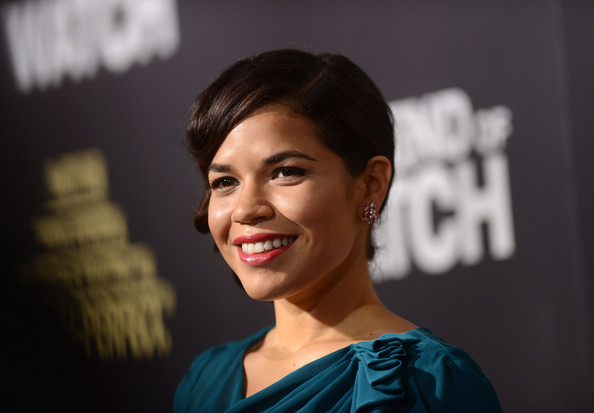
\includegraphics[width=\linewidth]{ferrera154}
			\caption{America Ferrera}
		\end{subfigure}
		\begin{subfigure}{0.33\linewidth}
			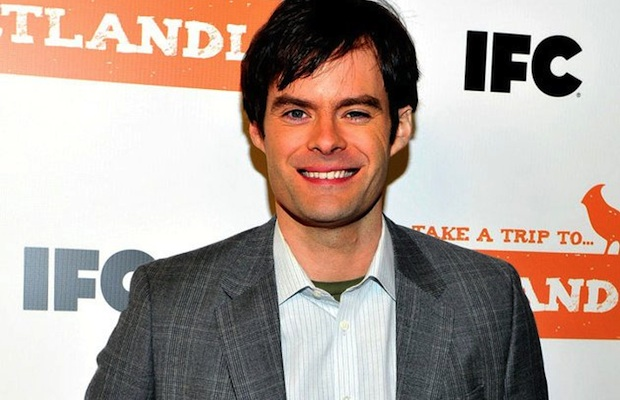
\includegraphics[width=\linewidth]{hader60}
			\caption{Bill Hader}
		\end{subfigure}
		\begin{subfigure}{0.33\linewidth}
			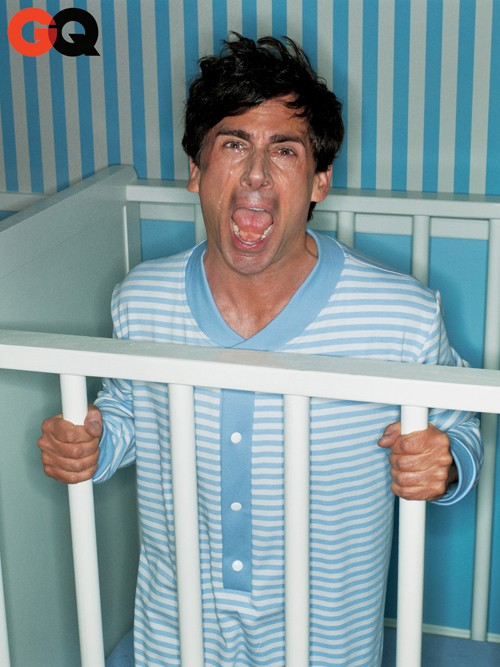
\includegraphics[width=\linewidth]{carell36}
			\caption{Steve Carell}
		\end{subfigure}
		\caption{Three examples of raw images in the dataset.}
		\label{fig:uncropped}
	\end{figure}

	\begin{figure}
		\begin{subfigure}{0.33\linewidth}
			
\includegraphics[width=\linewidth]{c_ferrera154}
			\caption{America Ferrera}
		\end{subfigure}
		\begin{subfigure}{0.33\linewidth}
			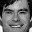
\includegraphics[width=\linewidth]{c_hader60}
			\caption{Bill Hader}
		\end{subfigure}
		\begin{subfigure}{0.33\linewidth}
			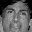
\includegraphics[width=\linewidth]{c_carell36}
			\caption{Steve Carell}
		\end{subfigure}
		\caption{Three examples of cropped images in the dataset, matching the examples provided in \cref{fig:uncropped}.}
		\label{fig:cropped}
	\end{figure}
\end{problem}
\clearpage

%----------------------------------------------------------------------------------------
%	PART 2
%----------------------------------------------------------------------------------------

\begin{problem}
	Creating the random training, validation, and testing sets was done in two steps. First, a random non-overlapping subset of the available images is selected. This is done directly through NumPy's choose function, but can also be implemented very simply without it. One example of an alternative method would be to randomly select then remove elements from the list of valid images. Since the order of the elements selected is randomly determined, there should be no correlation between an image and its position in the list of selected images. Thus, these elements are distributed between the three desired sets based on their index.
\end{problem}
\clearpage

%----------------------------------------------------------------------------------------
%	PART 3
%----------------------------------------------------------------------------------------

\begin{problem}
	In performing gradient descent for linear regression, the mean squared error was minimized:
	\begin{equation*}
		J(\theta) = \frac{1}{m}\sum_i \qty(\theta^\mathsf{T}x^{(i)} - y^{(i)})^2
	\end{equation*}
	where \(m\) is the number of images. The mean squared error was chosen as opposed to the squared error to ensure that the magnitude of the gradient would not increase as a function of the size of the training set, thus allowing the same learning rate to be used regardless of the size of the training set.
	
	The learning rate was selected to be as large as possible while maintaining the stability of the algorithm. If \(\alpha\) is too large, then taking a step during gradient descent will place the current position further up the gradient on the other side, resulting in the runaway growth of the parameters. If \(\alpha\) is too small (or slightly too large) however, the only issue may be that the algorithm would take a very long time to converge. Considering this, the learning rate was only selected to the nearest order of magnitude to minimize the validation error, settling on \num{e-3}. 
	
	The target epsilon for the desired change in \(\theta\) before finishing descent was selected in a very similar manner, settling on \num{4e-5}. A bound on the maximum number of iterations was set to \num{e5} to ensure that the optimization concluded in a timely manner. As recommended in the assignment instructions, the images were converted to have values to values between 0 and 1, allowing for the learning rate and final \(\theta\) to have reasonably sized values.
	
	With these choices the optimization produced a final testing error of 0.01584 and a final validation error of 0.04005. These two errors are reasonably similar in magnitude, suggesting that overfitting is not a large problem. The parameters obtained produced a \(100\%\) accuracy on classifying the images in the validation set and a \(95\%\) accuracy on classifying images in the training set.
	
	Below is a reduced version of the function used to compute the output of the classifier. Reduced in this context means that several lines of code related to later parts of this assignment were removed as they are not relevant here, but there were no changes to the lines present. While technically this function is used to compute the labelling accuracy, by providing only one image for the data parameter and simply 1 for the real\_labels parameter, the output of this function can be interpreted as a boolean. As described above and as implemented in main.py, the function will return True if this picture is Alec Baldwin and False if it is Steve Carell.
	
	\begin{minted}[mathescape,
		linenos,
		numbersep=5pt,
		gobble=2,
		frame=lines,
		framesep=2mm,
		tabsize=4,
		breaklines]{python}
		def labelling_accuracy(data, real_labels, parameters):
			results = np.dot(data, parameters[1:]) + parameters[0]
			return np.sum((results > 0.5) == real_labels) / len(real_labels)
	\end{minted}
	
\end{problem}
\clearpage

%----------------------------------------------------------------------------------------
%	PART 4
%----------------------------------------------------------------------------------------
\FloatBarrier
\begin{problem}
\begin{subproblem}
	The two sets of parameters are visualized in \cref{fig:4a}.
	\begin{figure}
		\begin{subfigure}{0.5\linewidth}
			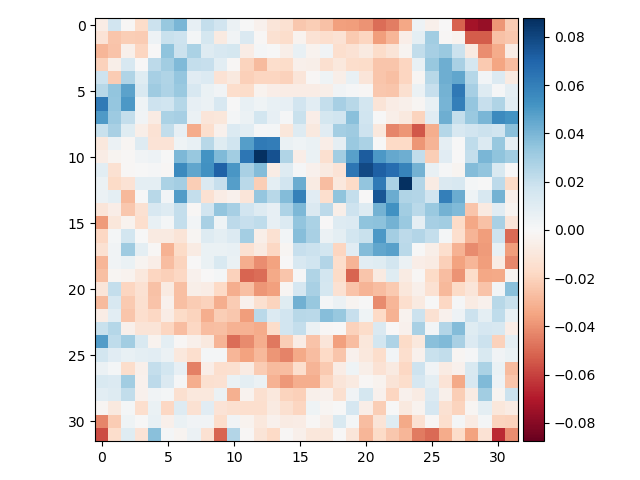
\includegraphics[width=\linewidth]{4a-1}
			\caption{Full training set}
		\end{subfigure}
		\begin{subfigure}{0.5\linewidth}
			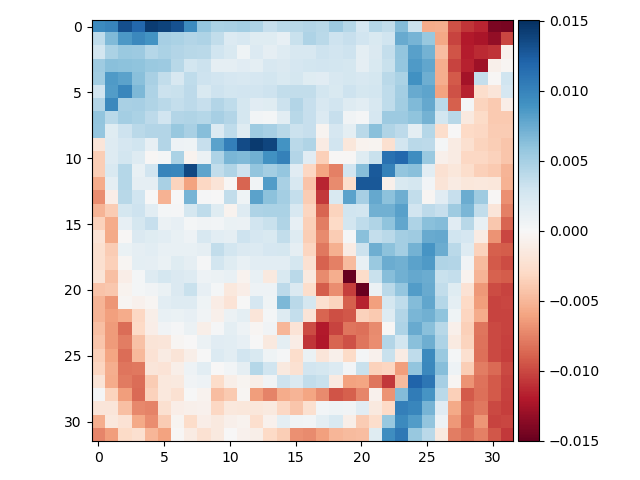
\includegraphics[width=\linewidth]{4a-2}
			\caption{Two images per actor}
		\end{subfigure}
	\caption{Visualization of the parameters obtained for the linear regression performed on a full training set and performed on a training set containing only two images per actor. The results from the smaller training have several sharp boundaries and odd features on an otherwise human looking face, suggesting that there is overfitting to specific features present in this smalller set.}
	\label{fig:4a}
	\end{figure}
\end{subproblem}
\begin{subproblem}
	The two kinds of images produced are show in \cref{fig:4b}. The more human like image was obtained by running gradient descent for only a small number of iterations (\num{100}), while the more random looking image was obtained by running for a very large number of iterations (\num{100000}). 
	
	Often in image recognition, the parameters end up highlighting specific features that are being used to differentiate. When they look random and have very sharp changes in weight, it may be an example of overfitting as the optimization focuses on specific pixels. Meanwhile, after only a small number of generations the parameter values will tend to move in a generally constant direction. The amount they move is scaled by the intensity of the image, so it will tend to produce a visualization of the "average" picture.
	\begin{figure}
		\begin{subfigure}{0.5\linewidth}
			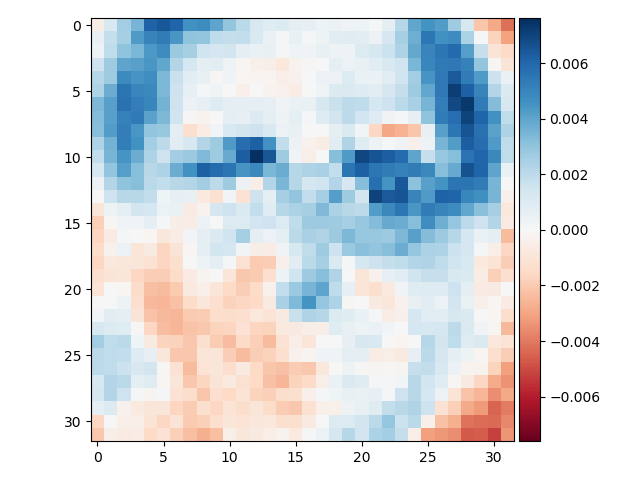
\includegraphics[width=\linewidth]{4b-1}
			\caption{\num{100} iterations}
		\end{subfigure}
		\begin{subfigure}{0.5\linewidth}
			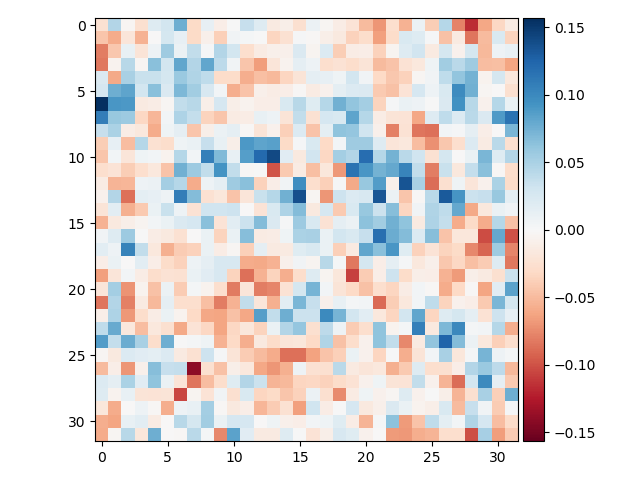
\includegraphics[width=\linewidth]{4b-2}
			\caption{\num{100000} iterations}
		\end{subfigure}
		\caption{Visualization of the parameters obtained for the linear regression for a varying number of generations.}
		\label{fig:4b}
	\end{figure}
\end{subproblem}
\end{problem}
\clearpage

%----------------------------------------------------------------------------------------
%	PART 5
%----------------------------------------------------------------------------------------

\FloatBarrier
\begin{problem}
	The performance of the classifier versus the size of the training set is shown in \cref{fig:5a}. Note that, as expected the performance on the training and validation sets increases as the size of the training set increases. This increase is fast at first, but slows down as the size of the training set increase; each additional image added does less to improve performance that the previous image.
	\begin{figure}
		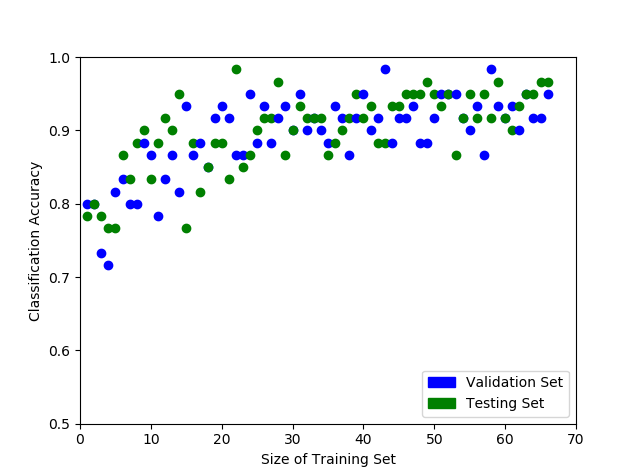
\includegraphics[width=\linewidth]{5}
		\caption{Performance of classifier versus size of training set on both the validation and testing set. Note that this figure was obtained with a random seed for each set size.}
		\label{fig:5a}
	\end{figure}
	
	On the full set, the individual actors were correctly classified as male or female with almost perfect accuracy:
	\begin{itemize}
		\item Lorraine Bracco classified with 1.0 accuracy
		\item Peri Gilpin classified with 0.98 accuracy
		\item Angie Harmon classified with 1.0 accuracy
		\item Alec Baldwin classified with 1.0 accuracy
		\item Steve Carell classified with 1.0 accuracy
		\item Bill Hader classified with 0.96 accuracy
	\end{itemize}
	Meanwhile, for the actors not in the training set, the accuracy ranged from great to not very good:
	\begin{itemize}
		\item Kristin Chenoweth classified with 0.64 accuracy
		\item America Ferrera classified with 0.92 accuracy
		\item Fran Drescher classified with 0.92 accuracy
		\item Gerard Butler classified with 0.96 accuracy
		\item Michael Vartan classified with 0.74 accuracy
		\item Daniel Radcliffe classified with 0.7 accuracy
	\end{itemize}
	This is likely the result of the overfitting of the classifier on the training set, focusing on features common to the specific actors rather than the features distinguishing male from female.
\end{problem}
\clearpage

%----------------------------------------------------------------------------------------
%	PART 6
%----------------------------------------------------------------------------------------

\begin{problem}
	\begin{subproblem}
		\begin{align*}
			\pdv{J(\theta)}{\theta_{pq}} &= \pdv{\theta_{pq}} \sum_i \qty(\sum_j\qty(\theta^\mathsf{T}x^{(i)} - y^{(i)})^2_j) \\
			&= \pdv{\theta_{pq}} \sum_i \qty(\theta_{pq} x^{(i)}_p - y^{(i)}_q)^2 \\
			&= 2 \sum_i x^{(i)}_p\qty(\theta_{pq} x^{(i)}_p - y^{(i)}_q) \numberthis \label{eq:dj}
		\end{align*}
	\end{subproblem}

	\begin{subproblem}
		Let \(X \in \mathbb{R}^{1025 \cross m}\) represent the training set with additional ones, where each column represents one image and \(m\) is the number of images. Let \(Y \in \mathbb{R}^{n \cross m}\) represent the labels  assigned to each image, with each column denoting one label and \(n\) being the number of actors to classify. Let \(\theta \in \mathbb{R}^{1025 \cross n}\) represent the parameters used for the linear regression.
		By the definition of the gradient,
		\begin{equation*}
			\grad{J(\theta)} = \pdv{J(\theta)}{\theta} = \begin{bmatrix}
				\pdv{J(\theta)}{\theta_{11}} & \cdots & \pdv{J(\theta)}{\theta_{1q}} \\
				\vdots & \ddots & \vdots \\
				\pdv{J(\theta)}{\theta_{p1}} & \cdots & \pdv{J(\theta)}{\theta_{pq}}
			\end{bmatrix}
		\end{equation*}
		Let \(\chi_p \in \mathbb{R}^{1 \cross m}\) represent the \(p\)-th row of \(X\) and let \(\gamma_q \in \mathbb{R}^{1 \cross m}\) represent the \(q\)-th row of \(Y\). \Cref{eq:dj} can thus be rewritten as:
		\begin{equation} \label{eq:dj2}
			\pdv{J(\theta)}{\theta_{pq}} = 2 \chi_p \qty(\theta_{pq}\chi_p - \gamma_q)^\mathsf{T}
		\end{equation}
		Let \(\theta^{(q)} \in \mathbb{R}^{1025 \cross 1}\) represent the \(q\)-th column of \(\theta\). Then, using \cref{eq:dj2}, 
		\begin{align*}
			\pdv{J(\theta)}{\theta^{(q)}} &= \begin{bmatrix} \pdv{J(\theta)}{\theta_{1q}} & \cdots & \pdv{J(\theta)}{\theta_{pq}} \end{bmatrix}^\mathsf{T} \\
			&= 2 X \qty(\qty(\theta^{(q)})^\mathsf{T}X - \gamma_q)^\mathsf{T}
		\end{align*}
		By the same process, the matrix is expanded along \(q\), obtaining the desired final expression:
		\begin{equation} \label{eq:grad}
			\grad{J(\theta)} = \pdv{J(\theta)}{\theta} = 2 X \qty(\theta^\mathsf{T}X - Y)^\mathsf{T}
		\end{equation}
	\end{subproblem}

	\begin{subproblem}
		For the reasons described in Part 3, the mean squared error is preferred. Additionally, it is more convenient to express the images as row vectors rather than column vectors. For these reasons, \cref{eq:grad} is modified by dividing by the number of images (\(m\)) and taking its transpose. Thus, the equation implemented is:
		\begin{equation}
			\pdv{J(\theta)}{\theta} = \frac{2}{m} X^\mathsf{T} \qty(X \theta - Y)
		\end{equation}
		
		This is implemented below,, along with the cost function. Note that in this implementation, \(X\) is not extended with additional ones but rather only multiplied with the relevant part of \(\theta\).	
		\begin{minted}[mathescape,
			linenos,
			numbersep=5pt,
			gobble=3,
			frame=lines,
			framesep=2mm,
			tabsize=4,
			breaklines]{python}
			def cost_function(data, labels, parameters):
				cost = np.linalg.norm(np.dot(data, parameters[1:]) + parameters[0] - labels)
				return cost ** 2 / len(data)
			
			def cost_gradient(data, labels, parameters):
				temp = np.dot(data, parameters[1:]) + parameters[0] - labels
				gradients = np.empty_like(parameters)
				gradients[0] = np.sum(temp)
				gradients[1:] = np.dot(data.T, temp)
				return 2 * gradients / len(data)
		\end{minted}
	\end{subproblem}

	\begin{subproblem}
		The code used to compare gradient descent algorithm above to the results obtained by finite differences is provided below:
		\begin{minted}[mathescape,
			linenos,
			numbersep=5pt,
			gobble=3,
			frame=lines,
			framesep=2mm,
			tabsize=4,
			breaklines]{python}
			# initialize some data to be used and find gradient
			images = get_data.load_data('bracco', [40])
			param = np.random.random((1025, 6)) * 1e-2
			labels = np.array([[1, 0, 0, 0, 0, 0]] * 40)
			grad = classifier.cost_gradient(images, labels, param)
			h = 1e-6
			# compare against finite differences
			np.random.seed(17)
			for _ in range(5):
				p = np.random.randint(0, 1025)
				q = np.random.randint(0, 6)
				param_mod = param.copy()
				param_mod[p, q] += h
				estimate = (classifier.cost_function(images, labels, param_mod) - classifier.cost_function(images, labels, param)) / h
				print('(p,q) =', (p, q), '-> function:', '{:f}'.format(grad[p, q]), '\t', 'estimate:', '{:f}'.format(estimate))
		\end{minted}
		
		By incrementing the element of the parameters at \((p,q)\) by \(h\) and then using the finite difference approximation, the gradient of the element at \((p,q)\) is approximated. Thus, by comparing this result to the value at the position \((p,q)\) of the result from from the gradient descent function function, we can attempt to see if the approximation matches what would be expected from the derived result. 
		
		In this case, with an \(h\) of \num{e-6} the values are accurate to at least seven significant figures, suggesting that the formula for the gradient descent found is correct. A smaller \(h\) would lead to even more accurate results, up to a certain limit of machine precision. The value above was selected since it is the smallest order of magnitude for which the the two values completely match in the standard python formatted float output.
	\end{subproblem}
\end{problem}
\clearpage

%----------------------------------------------------------------------------------------
%	PART 7
%----------------------------------------------------------------------------------------

\begin{problem}
	The parameters chosen for the gradient descent were the same as those described in Part 3, for the same reasons. Since the only practical difference is the number of images and since a error per image is used, it would make sense that there would not be any change needed in the parameters. With these choices, the classifier achieved a 0.8167 accuracy on both the validation and  training set for selecting the right actor out of the six possible choices.
	
	To find the label associated with the output of the classifier, the argmax of each row is found. The actor whose label has a one in this position and a zero in the other positions is then the corresponding actor associated with this output.
\end{problem}
\clearpage

%----------------------------------------------------------------------------------------
%	PART 8
%----------------------------------------------------------------------------------------

\FloatBarrier
\begin{problem}
	The parameters are visualized in \cref{fig:8}.
	\begin{figure}
		\begin{subfigure}{0.33\linewidth}
			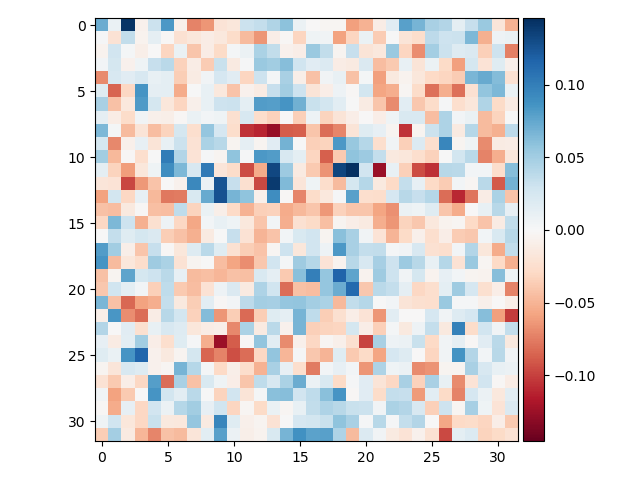
\includegraphics[width=\linewidth]{8-0}
			\caption{Lorraine Bracco}
		\end{subfigure}
		\begin{subfigure}{0.33\linewidth}
			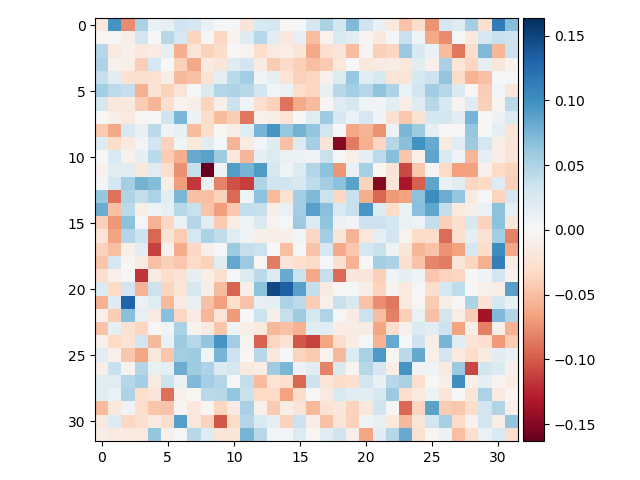
\includegraphics[width=\linewidth]{8-1}
			\caption{Peri Gilpin}
		\end{subfigure}
		\begin{subfigure}{0.33\linewidth}
			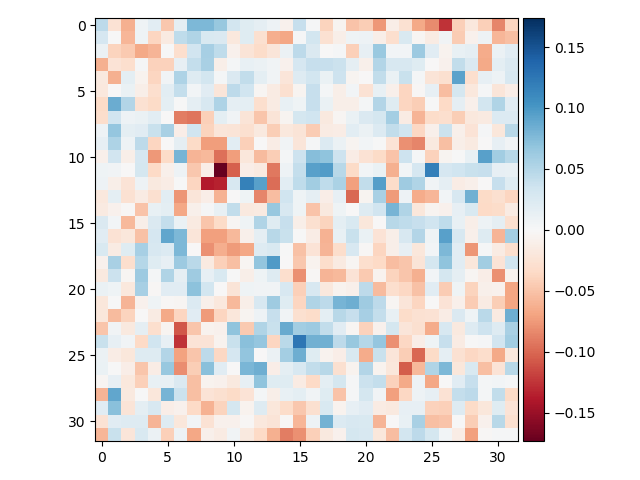
\includegraphics[width=\linewidth]{8-2}
			\caption{Angie Harmon}
		\end{subfigure}
		\begin{subfigure}{0.33\linewidth}
			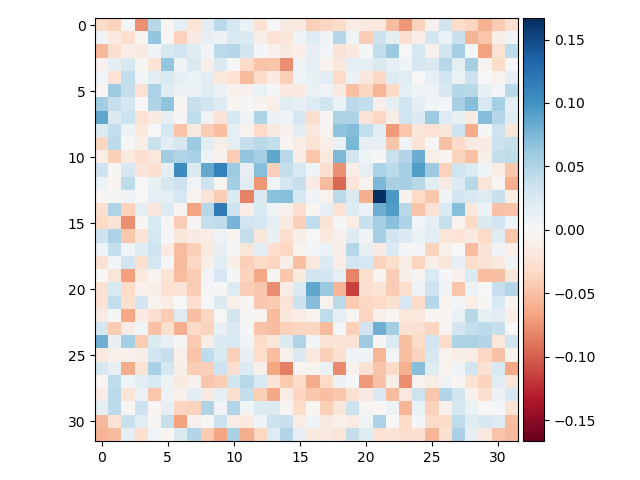
\includegraphics[width=\linewidth]{8-3}
			\caption{Alec Baldwin}
		\end{subfigure}
		\begin{subfigure}{0.33\linewidth}
			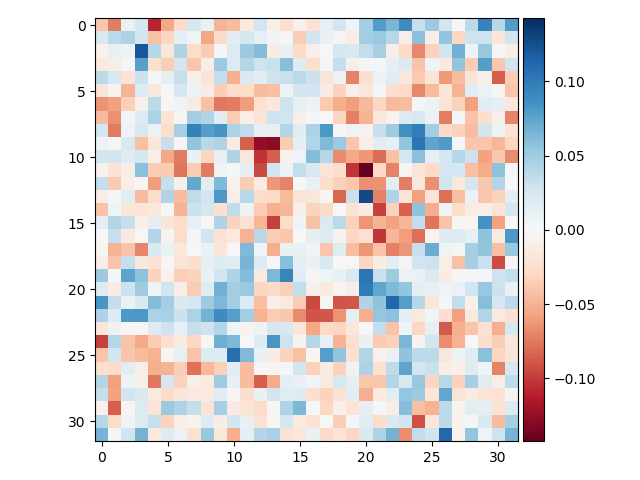
\includegraphics[width=\linewidth]{8-4}
			\caption{Steve Carell}
		\end{subfigure}
		\begin{subfigure}{0.33\linewidth}
			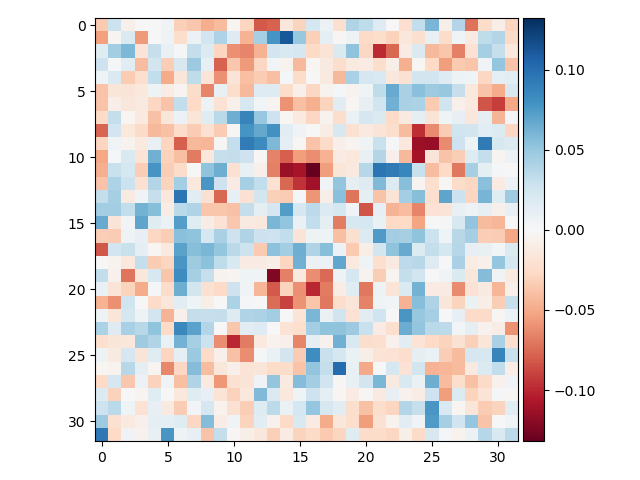
\includegraphics[width=\linewidth]{8-5}
			\caption{Alec Baldwin}
		\end{subfigure}
		\caption{Visualization of the parameters obtained for classification between the six different actors.}
		\label{fig:8}
	\end{figure}
	
\end{problem}
\clearpage

%----------------------------------------------------------------------------------------

\end{document}